%!TEX TS-program = xelatex
%!TEX root = ../../maxwell2018thesis.tex

\chapter[Modelling~\gls{acr:serp} Level Stopping Behaviours]{Modelling~\gls{acr:serp} Level\\Stopping Behaviours}\label{chap:serp}
In Chapters~\ref{chap:snippets} and~\ref{chap:diversity}, we examined the effects of searcher behaviour and performance when experimental interfaces and conditions were varied. This was before proceeding to examine the grounded simulated behaviour and performance of searchers under different snippet level stopping strategies. With the aforementioned considered as the empirical strand of the work reported in this thesis, \blueboxbold{HL-RQ1}\footnote{\blueboxbold{HL-RQ1} is defined in Section~\ref{sec:intro:rqs} on page~\pageref{sec:intro:rqs}.} poses the following overarching research question.

\begin{itemize}
    \item[]{\blueboxbold{HL-RQ1} How can we improve the current state-of-the-art searcher model to incorporate different points where individuals subscribing to such a model can stop?}
\end{itemize}

In order to address this high level research question, we presented in Chapter~\ref{chap:csm} the~\glsfirst{acr:csm}, a conceptual, high level model of the search process. The~\gls{acr:csm} introduced the~\gls{acr:serp} level stopping decision point, motivated by informations scent (refer to Section~\ref{sec:stopping_background:models:theoretical:ift}), allowing simulated searchers subscribing to such a model to \emph{abandon} a~\gls{acr:serp} if a general \emph{overview} of the given~\gls{acr:serp} if the results, from a glance, did not appear to provide promising results. With the definition of the~\gls{acr:csm} partially satisfying \blueboxbold{HL-RQ1}, we in this chapter provide results of an empirical, simulated study of the new stopping decision point, providing evidence that the inclusion of this new stopping decision point does indeed improve simulated searcher performance, and offers closer approximations to how real-world searchers actually behaved.

\section{Motivation and Research Questions}\label{sec:serp:background}
With the background work for this chapter largely outline in Sections~\ref{sec:stopping_background:models:theoretical:ift} and~\ref{sec:csm:new_stopping}, this section provides a refresher of the motivation behind the inclusion of the third, new~\gls{acr:serp} level stopping decision point. We begin with the concept of~\gls{acr:serp} abandonment, before considering how~\glsfirst{acr:ift} provides strong theoretical motivation.

The concept of the new~\gls{acr:serp} level stopping decision point revolves around the concept of~\gls{acr:serp} abandonment, when a searcher fails to click on any of the results returned for a given query~\citep{diriye2012abandonment, hassan2013serp_abandonment}. This may be for a variety of different reasons (both good and bad) -- the primary motivator for this study considers the notion of bad abandonment, where searchers abandon a~\gls{acr:serp} because they are dissatisfied by the results returned~\citep{hassan2013serp_abandonment}.

\begin{figure}[t!]
    \centering
    \resizebox{1\hsize}{!}{
    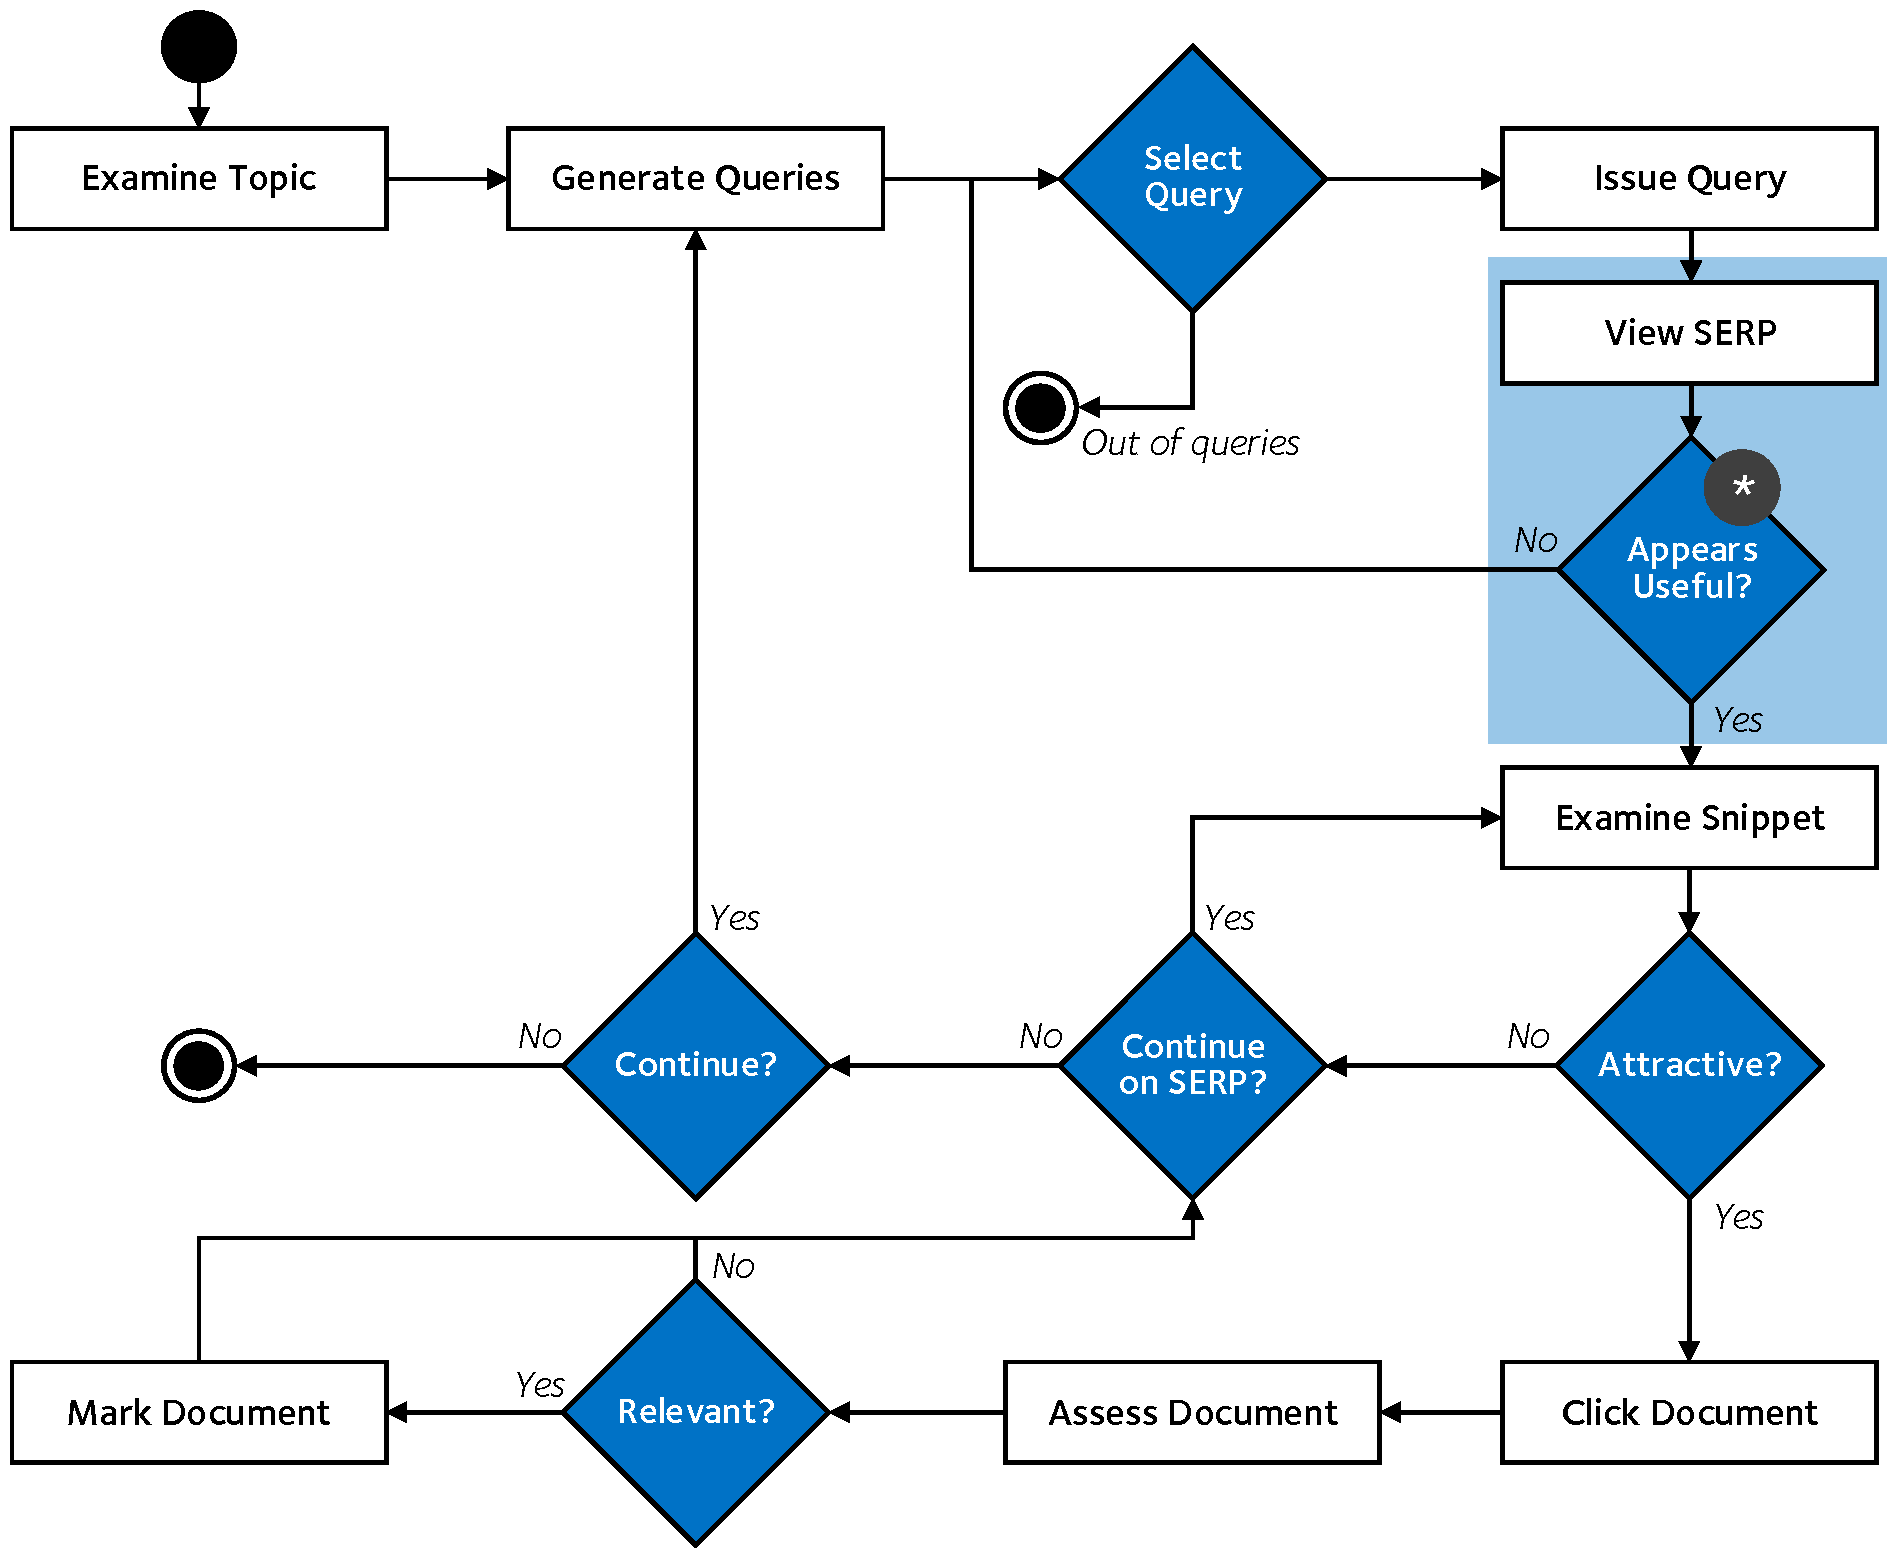
\includegraphics{figures/ch9-csm.pdf}}
    \caption[The~\glsfirst{acr:csm} and~\gls{acr:serp} stopping point]{The~\glsfirst{acr:csm}, highlighting the stopping decision point (by an asterisk\emph{*}, with the~\gls{acr:serp} examination component also highlighted within the blue rectangle) that is examined in detail in this chapter. Refer to Section~\ref{sec:csm:csm:flow} for an in-depth explanation of the model.}
    \label{fig:csm_ch9}
\end{figure}

Motivated by \emph{information scent} and the \emph{patch model} -- both part of~\glsfirst{acr:ift}\footnote{Refer to Section~\ref{sec:stopping_background:models:theoretical:ift} on page~\pageref{sec:stopping_background:models:theoretical:ift} for a detailed explanation of the patch model.} --~\cite{pirolli1999ift} argue that information seekers are like animals foraging in the wild, and as such will follow a scent to find food. As discussed previously, information seekers have been shown to follow a series of \emph{proximal cues} provided by~\gls{acr:serp} components such as hypertext links, titles, snippets and thumbnails to help locate relevant information~\citep{pirolli1995ift, pirolli1999ift, chi2001information_scent, oltston2003scenttrails, pirolli2007ift}. For example,~\cite{card2001scent_graphs} found that when navigating through webpages, searchers were more likely to leave when the information scent provided on a page began to decline. Work by~\cite{wu2014information_scent} discussed a user study where low, medium and high scent~\glsplural{acr:serp} were created by changing the number and distribution of relevant items on the page -- thus altering the proximal cues provided. Those interacting with high scent~\glsplural{acr:serp} examined more content and went to greater depths compared to those who utilised low scent~\glsplural{acr:serp}. Further work by~\cite{ong2017scent_behaviour} -- and indeed the user study reported in Section~\ref{chap:snippets:user} -- all confirm that modifying the scent of a~\gls{acr:serp} does indeed alter a searcher's stopping behaviour.

For this chapter, we operationalise the information scent as the performance of a given~\gls{acr:serp}, examining how the new~\gls{acr:serp} level stopping decision point within the searcher model -- as shown in Figure~\ref{fig:csm_ch9}\footnote{Further information on the~\glsfirst{acr:csm} can be found in Chapter~\ref{chap:csm}, starting on page~\pageref{chap:csm}.} -- affects searcher, stopping and overall performance. This is achieved by enumerating a series of different~\gls{acr:serp} level stopping strategies, allowing us to operationalise the new stopping decision point in several ways. As such, we pose two key research questions to be addressed in this chapter.

\begin{itemize}
    \item[]{\blueboxbold{RQ1} Does incorporating a~\gls{acr:serp} level stopping decision point lead to higher overall performance?}
    \item[]{\blueboxbold{RQ2} Does incorporating a~\gls{acr:serp} level stopping decision point lead to better approximations of searcher stopping behaviour?}
\end{itemize}

Taken together, the answers to these research questions will in turn provide a complete answer to allow us to address high level \blueboxbold{HL-RQ1}, allowing us to determine whether the inclusion of this additional~\gls{acr:serp} level stopping decision point does improve on the current state-of-the-art. In the next section, we outline the methodology undertaken to address the aforementioned research questions.

\section{Methodology}
In order to address the two research questions posed above, we followed our simulation methodology, outlined in our general methodology chapter. This is detailed in Section~\ref{chap:csm:method:simulation} on page~\pageref{chap:csm:method:simulation}. A variety of different simulation components that mapped to individual components of the~\gls{acr:csm} were left unchanged from the general methodology; this section details the changes to our experimental setup, the key component being the~\gls{acr:serp} level stopping decision point was operationalised for this study.

In this section, we therefore outline:

\begin{itemize}
    \item{the different~\gls{acr:serp} level stopping decision point strategies that were trialled, including the introduction of a new probability of examining a~\gls{acr:serp} (Section~\ref{sec:serp:method:serp_dp});}
    \item{a discussion of the different interaction probabilities and costs that were used for this study (Section~\ref{sec:serp:method:probscosts});}
    \item{an enumeration of the different snippet level stopping strategies trialled for this study (Section~\ref{sec:serp:method:snippet}); and}
    \item{a summary of the other components of the~\gls{acr:csm} that were instantiated in a different way as outlined in the general methodology (Section~\ref{sec:serp:method:other}).}
\end{itemize}

\subsection{\gls{acr:serp} Decision Making}\label{sec:serp:method:serp_dp}
This discusses the various ways in which we implemented this new stopping decision point, allowing us to determine whether it leads to any improvements in overall search performance and better approximations to real-world searcher stopping behaviours.

\blueboxbold{Definition: Low vs. High Scent} First, we must define our interpretation of how the scent of a~\gls{acr:serp} was measured. We follow the work of~\cite{wu2014information_scent}, who stated that a page offering little or no relevant content could be considered to offer a low information scent. As such, our definition of a poor quality~\gls{acr:serp} is defined as $P@10=0.0$. We use this definition to delineate between \emph{good} and \emph{bad}~\glsplural{acr:serp} when considering interaction probabilities below.

\blueboxbold{Probability of Examination} For this new stopping decision point, we introduce the \emph{probability of examining a~\gls{acr:serp}}, or \blueboxbold{P(E)}. This determines how likely it is a searcher will \emph{enter} a~\gls{acr:serp} and begin to examine result summaries in detail. Taking this concept further, we can then consider two additional probabilities that incorporate the notion of a~\glsplural{acr:serp} information scent, yielding:

\begin{itemize}
    \item{\blueboxbold{P(E|HS)}, the probability of examining a~\gls{acr:serp} perceived to give a high information scent (i.e. a good quality~\gls{acr:serp}); and}
    \item{\blueboxbold{P(E|LS)}, the probability of examining a~\gls{acr:serp} offering what appears to be a low information scent (i.e. a poor quality~\gls{acr:serp}, or $P@10=0.0$).}
\end{itemize}

\begin{figure}[t!]
    \centering
    \resizebox{1\hsize}{!}{
    
\includegraphics{figures/ch6-serp_probabilities.pdf}}
    \caption[Computing~\gls{acr:serp} examination probabilities]{A simple illustration highlighting how the different~\gls{acr:serp} examination costs were computed. We consider both the probability of examining~\glsplural{acr:serp} yielding both high and low information scents. Definitions are used from~\cite{wu2014information_scent} and~\cite{hassan2013serp_abandonment}.}
    \label{fig:serp_probabilities}
\end{figure}

These values were computed from interaction log data, derived from the two user studies discussed in Chapters~\ref{chap:snippets} and~\ref{chap:diversity}. Values derived are not reported in this section; refer to Section~\ref{sec:serp:method:probscosts} for the probabilities extracted. Intuitively however, one would expect a searcher demonstrating competency at searching for information to know when a query is returning good results, and vice versa. As such, one would expect to see a higher probability for $P(E|HS)$ than when compared to $P(E|LS)$, and would thus provide evidence that searchers do indeed attempt to avoid low quality~\glsplural{acr:serp}.

As illustrated in Figure~\ref{fig:serp_probabilities}, we took each query issued from the interaction log, and extracted for each the $P@10$ score (as per~\cite{wu2014information_scent}). If $P@10=0.0$, the associated~\gls{acr:serp} for the query would have offered a low information scent. Conversely, if $P@10 > 0.0$, the information scent would have been considered to be high. For the interactions recorded on each~\gls{acr:serp}, we could then count the number that recorded no clicks (or no result summaries deemed to be attractive enough to examine further). We considered this as a definition of an \emph{abandoned~\gls{acr:serp}}, as used in previous work by~\cite{hassan2013serp_abandonment}. From these counts, we could then compute the probabilities of examining a~\gls{acr:serp}, as illustrated in Figure~\ref{fig:serp_probabilities}.

\blueboxbold{Considering Browser Viewport Size}
We now turn our attention to how a simulated searcher is able to make a judgement of the presented~\gls{acr:serp}. As we discussed previously in Section~\ref{sec:serp:background}, real-world searchers are able to infer the quality (and perhaps relevance) of a given page or~\gls{acr:serp} through the examination of various proximal cues~\citep{chi2001information_scent}.

\begin{wrapfigure}[13]{r}{0.45\textwidth}
    \begin{center}
    \vspace*{-9mm}
    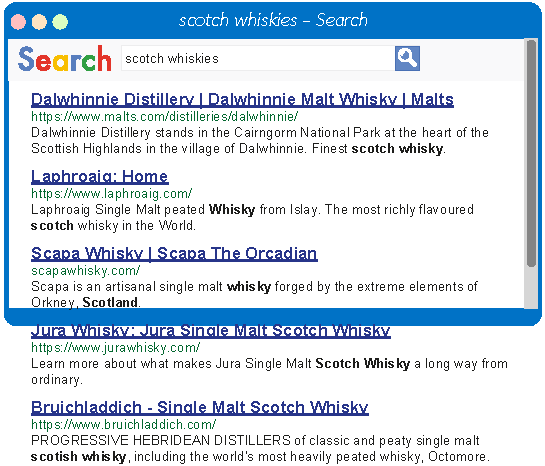
\includegraphics[width=1\textwidth]{figures/ch6-viewport.pdf}
    \end{center}
    \vspace*{-2mm}
    \caption[Viewport cutoff example]{The~\gls{acr:serp} viewport threshold. In this example, three result summaries are visible, with two present but outwith the viewport. Therefore, \emph{v\textsubscript{size}=3}. Cheers!}
    \label{fig:viewport_cutoff}
\end{wrapfigure}

While we do not specifically examine different cues, instead relying on more simplistic means to operationalise the stopping decision point, we nevertheless do consider the \emph{size of the browser's viewport}. A~\gls{acr:serp} is typically larger than the viewport it is displayed within, which leads to the inclusion of scrollbars. Results can only be seen \emph{above-the-fold}, or what is visible within the viewport. We argue that a searcher can infer the quality of the~\gls{acr:serp} from the initial view they are presented with, and thus incorporate a \emph{viewport size} ($v_{size}$) variable in our implementations. A searcher can only judge what they can see. This variable can vary between the different interfaces we trialled -- for example, longer snippet text results in fewer result summaries being displayed in the initial view. By using a fixed-size popup window in the two user studies (as discussed in Section~\ref{sec:csm:methodology:user:interface}), we were then able to manually check the number of result summaries displayed within the popup window, and use these values to ground the new stopping decision point further.

For our simulations, we use different values of $v_{size}$ over the study interfaces reported in Chapter~\ref{chap:snippets} only. This is because introducing longer result summaries would mean fewer overall would be displayed within a viewport of the same size. Across the experimental conditions trialled in Chapter~\ref{chap:diversity}, $v_{size}$ remains constant as result summary lengths were not modified. Values used for $v_{size}$ are reported later in Section~\ref{sec:serp:method:probscosts}.

\subsubsection{Decision Point Implementations}\label{sec:serp:method:serp_dp:implementations}
We trialled three different implementations of the~\gls{acr:serp} level stopping decision point, providing us with the ability to determine the effect of incorporating it within the~\gls{acr:csm}. These are enumerated below, with an explanation of each. The first can be considered our simple baseline approach.

\begin{itemize}
    \item{\blueboxbold{Always Examine (Baseline)} With this approach, a searcher will \emph{always enter} the~\gls{acr:serp}, and examine at least one result summary -- the exact number would be determined by the snippet level stopping strategy. This is the current state-of-the-art, and we consider this as our baseline. Indeed, this strategy was used in the simulations reported in Chapters~\ref{chap:snippets} and~\ref{chap:diversity}.}
\end{itemize}

From here, the remaining two strategies begin to consider a simulated searcher's judgements regarding the perceived quality of a~\gls{acr:serp}, and thus begin to use the new stopping decision point to abandon a~\gls{acr:serp} before examining individual result summaries in detail.

\begin{itemize}
    \item{\blueboxbold{Perfect~\gls{acr:serp} Judgements} Here, a simulated searcher will only begin to examine a~\gls{acr:serp} in detail if $P@v_{size} > 0$ (considering the viewport size). If $P@v_{size} = 0$, the searcher will abandon the~\gls{acr:serp}, and proceed to the next action as dictated by the~\gls{acr:csm}. This is the upper bound in terms of performance for the stopping decision point, and is analogous to, as an example, the \emph{ideal user} of~\cite{hagen2016simulating_users}.}
    \item{\blueboxbold{Stochastic~\gls{acr:serp} Judgements} This implementation used a stochastic element to determine whether the simulated searcher should enter the~\gls{acr:serp} or not. Like above, the viewport size ($P@v_{size}$) of the~\gls{acr:serp} is computed. If the~\gls{acr:serp} is of high scent, $P(E|HS)$ is used to determine whether the searcher should enter the~\gls{acr:serp}. Conversely, if the~\gls{acr:serp} is considered to be of low scent, $P(E|LS)$ is used instead to determine the likelihood of abandonment. We considered three different sets of probabilities for the stochastic implementation.}
    
    \begin{itemize}
        \item{\blueboxbold{Average} $P(E|HS)$ and $P(E|LS)$ are estimated over all subjects of a particular interface or condition.}
        \item{\blueboxbold{Savvy} $P(E|HS)$ and $P(E|LS)$ are estimated based upon the top 15 subjects for a particular interface/condition with the \emph{lowest} $P(E|LS)$.}
        \item{\blueboxbold{Na\"{i}ve} $P(E|HS)$ and $P(E|LS)$ are estimated based upon the top 15 subjects for a particular interface/condition with the \emph{highest} $P(E|LS)$.}
    \end{itemize}
\end{itemize}

By considering these different approaches to implementing the new~\gls{acr:serp} level stopping decision point, we can then clearly identify whether it can offer improved performance and approximations of actual searcher stopping behaviours. We also run each of the stochastic~\gls{acr:serp} level stopping decision components a total of \todo{$30$} times, computing the average over the different trials.

\subsection{Interfaces, Conditions, and Experimental Grounding}\label{sec:serp:method:probscosts}
To determine whether the new~\gls{acr:serp} level stopping decision points offers improvements across a variety of different interfaces and conditions (and can therefore considered to be generalisable), we conducted a series of simulations across the eight interface and experimental conditions trialled in the two user studies, reported in Chapters~\ref{sec:snippets} and~\ref{sec:diversity}.

\begin{table}[t!]
    \caption[Experimental interfaces and conditions]{Experimental interfaces and conditions trialled in this chapter, based upon the work reported in Chapters~\ref{chap:snippets} and~\ref{chap:diversity}. In total, eight different experimental interfaces and conditioned were trialled, considering different result summary lengths, systems and tasks.}
    \label{tbl:serp_conditions}
    \renewcommand{\arraystretch}{1.8}
    \begin{center}
    \begin{tabulary}{\textwidth}{L{0.4cm}@{\CS}L{3.2cm}@{\CS}D{3.51cm}@{\CS}D{3.51cm}@{\CS}D{3.51cm}@{\CS}}

        \RS & & \lbluecell \textbf{Summary Length} & \lbluecell \textbf{System} & \lbluecell \textbf{Task} \\

        \RS \multirow{4}{*}{\rotatebox{90}{\hspace*{-4mm}\textbf{Chapter~\ref{chap:snippets}}}} & \lbluecell\textbf{T0} & \cell \small{Title only} & \cell \small{\blueboxbold{ND} (Non Div.)} & \cell \small{\darkblueboxbold{AD} (Ad-hoc)}\\
        \RS & \lbluecell\textbf{T1} & \cell \small{Title + 1 snippet} & \cell \small{\blueboxbold{ND} (Non Div.)} & \cell \small{\darkblueboxbold{AD} (Ad-hoc)}\\
        \RS & \lbluecell\textbf{T2} & \cell \small{Title + 2 snippets} & \cell \small{\blueboxbold{ND} (Non Div.)} & \cell \small{\darkblueboxbold{AD} (Ad-hoc)}\\
        \RS & \lbluecell\textbf{T4} & \cell \small{Title + 4 snippets} & \cell \small{\blueboxbold{ND} (Non Div.)} & \cell \small{\darkblueboxbold{AD} (Ad-hoc)}\\
        
        \RS\RS\RS \multirow{4}{*}{\rotatebox{90}{\hspace*{-4mm}\textbf{Chapter~\ref{chap:diversity}}}} & \lbluecell\textbf{D-AS} & \cell \small{Title + 2 snippets} & \cell \small{\blueboxbold{D} (Div.)} & \cell \small{\darkblueboxbold{AS} (Aspectual)}\\
        \RS & \lbluecell\textbf{ND-AS} & \cell \small{Title + 2 snippets} & \cell \small{\blueboxbold{ND} (Non Div.)} & \cell \small{\darkblueboxbold{AS} (Aspectual)}\\
        \RS & \lbluecell\textbf{D-AD} & \cell \small{Title + 2 snippets} & \cell \small{\blueboxbold{D} (Div.)} & \cell \small{\darkblueboxbold{AD} (Ad-hoc)}\\
        \RS & \lbluecell\textbf{ND-AD} & \cell \small{Title + 2 snippets} & \cell \small{\blueboxbold{ND} (Non Div.)} & \cell \small{\darkblueboxbold{AD} (Ad-hoc)}\\
        
    \end{tabulary}
    \end{center}
\end{table}

From Chapter~\ref{chap:snippets}, the four different experimental interfaces -- whereby result summary lengths were manipulated -- are considered. Namely, these are \blueboxbold{T0}, \blueboxbold{T1}, \blueboxbold{T2} and \blueboxbold{T4}. From Chapter~\ref{chap:diversity}, we also considered the four experimental conditions that manipulated the underlying system and searcher tasks: \dualbluebox{D}{AS}, \dualbluebox{ND}{AS}, \dualbluebox{D}{AD} and \dualbluebox{ND}{AD}. The eight interfaces and conditions trialled are presented in Table~\ref{tbl:serp_conditions}, complete with an explanation of the differences between each.

\begin{table}[t!]
    \caption[Simulation interaction probabilities and v\textsubscript{size}]{Probabilities of examining high \emph{P(E|HS)} and low scent~\glsplural{acr:serp} \emph{P(E|LS)}, along with \emph{v\textsubscript{size}} values for each of the eight different experimental interfaces and conditions trialled, reported over three different set of probabilities. Refer to Tables~\ref{tbl:snippets_simulation_probcosts} (page~\pageref{tbl:snippets_simulation_probcosts}) and~\ref{tbl:diversity_simulation_probcosts} (page~\pageref{tbl:diversity_simulation_probcosts}) for other interaction probabilities and costs for studies reported in Chapters~\ref{chap:snippets} and~\ref{chap:diversity} respectively.}
    \label{tbl:serp_probs_costs}
    \renewcommand{\arraystretch}{1.8}
    \begin{center}
    \begin{tabulary}{\textwidth}{L{0.4cm}@{\CS}L{3.2cm}@{\CS}D{2.5cm}@{\CS}D{2.5cm}@{\CS}D{2.5cm}@{\CS}D{2.5cm}@{\CS}}

        \RS & \dbluecell \textbf{Chapter~\ref{chap:snippets}} & \lbluecell \textbf{T0} & \lbluecell \textbf{T1} & \lbluecell \textbf{T2} & \lbluecell \textbf{T4} \\
        
        \RS \multirow{2}{*}{\rotatebox{90}{\hspace*{-2mm}\textbf{Average}}} & \lbluecell\textbf{P(E|HS)} & \cell \small{xx} & \cell \small{xx} & \cell \small{xx} & \cell \small{xx}\\
        \RS & \lbluecell\textbf{P(E|LS)} & \cell \small{xx} & \cell \small{xx} & \cell \small{xx} & \cell \small{xx}\\
        
        \RS\RS\RS \multirow{2}{*}{\rotatebox{90}{\hspace*{-2mm}\textbf{Savvy}}} & \lbluecell\textbf{P(E|HS)} & \cell \small{xx} & \cell \small{xx} & \cell \small{xx} & \cell \small{xx}\\
        \RS & \lbluecell\textbf{P(E|LS)} & \cell \small{xx} & \cell \small{xx} & \cell \small{xx} & \cell \small{xx}\\
        
        \RS\RS\RS \multirow{2}{*}{\rotatebox{90}{\hspace*{-2mm}\textbf{Na\"{i}ve}}} & \lbluecell\textbf{P(E|HS)} & \cell \small{xx} & \cell \small{xx} & \cell \small{xx} & \cell \small{xx}\\
        \RS & \lbluecell\textbf{P(E|LS)} & \cell \small{xx} & \cell \small{xx} & \cell \small{xx} & \cell \small{xx}\\
        
        \RS\RS\RS & \lbluecell\textbf{v\textsubscript{size}} & \cell \small{xx} & \cell \small{xx} & \cell \small{xx} & \cell \small{xx}\\
        
        \RS\RS\RS\RS\RS\RS & \dbluecell \textbf{Chapter~\ref{chap:diversity}} & \lbluecell \textbf{D-AS} & \lbluecell \textbf{ND-AS} & \lbluecell \textbf{D-AD} & \lbluecell \textbf{ND-AD} \\
        
        \RS \multirow{2}{*}{\rotatebox{90}{\hspace*{-2mm}\textbf{Average}}} & \lbluecell\textbf{P(E|HS)} & \cell \small{xx} & \cell \small{xx} & \cell \small{xx} & \cell \small{xx}\\
        \RS & \lbluecell\textbf{P(E|LS)} & \cell \small{xx} & \cell \small{xx} & \cell \small{xx} & \cell \small{xx}\\
        
        \RS\RS\RS \multirow{2}{*}{\rotatebox{90}{\hspace*{-2mm}\textbf{Savvy}}} & \lbluecell\textbf{P(E|HS)} & \cell \small{xx} & \cell \small{xx} & \cell \small{xx} & \cell \small{xx}\\
        \RS & \lbluecell\textbf{P(E|LS)} & \cell \small{xx} & \cell \small{xx} & \cell \small{xx} & \cell \small{xx}\\
        
        \RS\RS\RS \multirow{2}{*}{\rotatebox{90}{\hspace*{-2mm}\textbf{Na\"{i}ve}}} & \lbluecell\textbf{P(E|HS)} & \cell \small{xx} & \cell \small{xx} & \cell \small{xx} & \cell \small{xx}\\
        \RS & \lbluecell\textbf{P(E|LS)} & \cell \small{xx} & \cell \small{xx} & \cell \small{xx} & \cell \small{xx}\\
        
        \RS\RS\RS & \lbluecell\textbf{v\textsubscript{size}} & \cell \small{xx} & \cell \small{xx} & \cell \small{xx} & \cell \small{xx}\\
        
    \end{tabulary}
    \end{center}
\end{table}

Table~\ref{tbl:serp_probs_costs} presents the probabilities of examining~\glsplural{acr:serp} yielding low ($P(E|LS)$) and high ($P(E|HS)$) scents. Values are computed as per the explanations provided in Section~\ref{sec:serp:method:serp_dp}. The table reports values across each of the eight different experimental interfaces and conditions trialled. In addition, values are reported for each interface and condition across the three different probability sets of \emph{average, savvy} and \emph{na\"{i}ve} searchers (as discussed in Section~\ref{sec:serp:method:serp_dp:implementations}). Also included within the table are the $v_{size}$ values used across each interface or condition, denoting the number of result summaries within a simulated viewport.

These values should be considered in tandem with the interaction costs and probabilities presented in Tables~\ref{tbl:snippets_simulation_probcosts} (presented on page~\ref{tbl:snippets_simulation_probcosts}) and~\ref{tbl:diversity_simulation_probcosts} (presented on page~\pageref{tbl:diversity_simulation_probcosts}) for other classical interaction probabilities (considering the probabilities of marking result summaries, $P(C|R)$ and $P(C|N)$ -- and saving documents, $P(S|R)$ and $P(S|N)$) and interaction costs (including the cost of: querying; examining a~\gls{acr:serp}; examining a result summary; examining a document; and saving a document) for the studies reported in Chapters~\ref{chap:snippets} and~\ref{chap:diversity} respectively. Table~\ref{tbl:serp_probs_costs} reports only the probabilities of examining a~\gls{acr:serp}.

\subsection{Snippet Level Stopping Strategies}\label{sec:serp:method:snippet}
Chapter~\ref{chap:strategies} presented thirteen different snippet level stopping strategies. To reduce the complexity of the experimentation reported in this chapter, we decided to reduce the number of snippet level stopping strategies that we considered. Doing so reduced the risk of potentially repeating the same results as shown before, while still demonstrating that when enabled, the~\gls{acr:serp} level stopping decision point yielded improved performance and closer approximations to actual searcher stopping behaviour over a range of configurations.

As such, we report over the following \todo{six} snippet level stopping strategies in this chapter. These were selected as they offered good performance and approximations of actual searcher stopping behaviours in results presented in previous chapters.

\begin{itemize}
    \item{\blueboxbold{SS1}}
    \item{\blueboxbold{SS2}}
    \item{\blueboxbold{SS3}}
    \item{\blueboxbold{SS4}}
    \item{\blueboxbold{SS5}}
    \item{\blueboxbold{SS6}}
\end{itemize}

Note that these strategies were instantiated with the same $x_n$ values as reported in the general methodology in Section~\ref{chap:csm:method:simulation:grounding:stopping_strats} on page~\pageref{chap:csm:method:simulation:grounding:stopping_strats}.

\subsection{Remaining~\gls{acr:csm} Components}\label{sec:serp:method:other}
We considered only the query generation strategy \blueboxbold{QS3\textsuperscript{+}}, as outlined in Section~\ref{chap:csm:method:simulation:grounding:querying} (page~\pageref{chap:csm:method:simulation:grounding:querying}) for use in the performance runs. This helped to simplify and reduce the number of experimental runs required. For comparison runs, queries issued by real-world subjects under each of the eight experimental interfaces and conditions were again \emph{replayed}, as discussed in Section~\ref{chap:csm:method:sim:runs:comparison} on page~\pageref{chap:csm:method:sim:runs:comparison}.

For the four experimental interfaces trialled in the study reported in Chapter~\ref{chap:snippets}, the same experimental methodology was followed as described in Section~\ref{sec:snippets:simulations:method}. Similarly, the same experimental method was followed as reported in Section~\ref{sec:diversity:simulated:method} for the four experimental conditions belonging to the studies reported in Chapter~\ref{chap:diversity}.

\section{Results}

\subsection{Performance Runs}

\subsection{User Comparison Runs}

\section{Discussion and Chapter Summary}